%!LW recipe=pdflatex-shellescape
\documentclass[11pt]{book}

\usepackage{geometry}
\geometry{margin=1in}

\usepackage[utf8]{inputenc}
%\usepackage[english]{babel}

\usepackage{graphicx}
\usepackage[dvipsnames]{xcolor}
\usepackage{amsmath}
\usepackage{float}
\usepackage{natbib}
\bibliographystyle{mnras}
\setcitestyle{authoryear,open={(},close={)}}
%\usepackage[hybrid]{markdown}
\usepackage{enumitem}
\setitemize{itemsep=-2pt}
\usepackage[colorlinks=true,allcolors=blue]{hyperref}
\usepackage{caption}
\usepackage{overpic}
\usepackage{amssymb}
\usepackage{multirow}
\usepackage{mathtools} 
\usepackage{lipsum}
\usepackage{fancyheadings}
\usepackage{tcolorbox}

\renewcommand{\subsectionmark}[1]{%
  \markright{\MakeUppercase{\thesubsection.\ #1}}}%

\pagestyle{fancy}
\fancyhead[L]{}
\fancyhead[R]{\nouppercase{\rightmark}}
\fancyfoot[R]{\vspace{-5pt}\rule{\textwidth}{0.4pt}\\ \thepage}
\fancyfoot[C]{\protect\color{gray}Compiled on \today}

\tcbset{textmarker/.style={%
        parbox=false,boxrule=0mm,boxsep=0mm,arc=0mm,
        outer arc=0mm,left=2mm,right=2mm,top=7pt,bottom=7pt,
        toptitle=1mm,bottomtitle=1mm,oversize}}
        
% define new colorboxes
% add breakable ?
\newtcolorbox[auto counter,number within=chapter]{hintBox}[1][]{textmarker, colback=yellow!10!white}
\newtcolorbox{importantBox}{textmarker, colback=red!10!white}
\newtcolorbox{noteBox}{textmarker, colback=green!10!white}

% define commands for easy access
\newcommand{\note}[2]{\begin{noteBox} \textbf{#1} #2 \end{noteBox}}
\newcommand{\warning}[2]{\begin{hintBox} \textbf{#1} #2 \end{hintBox}}
\newcommand{\important}[2]{\begin{importantBox} \textbf{#1} #2 \end{importantBox}}

\begin{document}

\tableofcontents
%\clearpage

\chapter{Previous notes from Cole}

\section{May 12th, 2022}

I'm starting a notebook because I keep forgetting what I'm working on. Hopefully this will complement the git logs.

Today I was able to update the \texttt{Ensemble} constructor function and write a function in \texttt{explore-parameters.jl} that will generate an Ensemble and run the dynamics. I need to check for bugs and work on the visualization side now.

I need to make sure to use \texttt{@quickactivate} with DrWatson; otherwise, saving does not work as expected.

\section{June 24th, 2022}

I should focus on this project a bit more. My goal today is to make a plan of attack. This should include a few different things, mostly issues on git to guide future development.\\

\textbf{Main goals:}

\begin{itemize}
    \item Parameter sweep of the well-mixed case:
    \begin{itemize}
        \item Plot Max MA, MA distribution fit, integer number against (forward, backward rate)
    \end{itemize}

    \item Parameter sweep of spatially distributed cases:
    \begin{itemize}
        \item Plot same things against diffusion rates
        \item Start with Line Graphs, then lattice, then random.
        \item Compute MA of Graphs. (Pick forward/backward rate from sweep above and vary diffusion)
    \end{itemize}
\end{itemize}

To do those we'll need a coherent data management system and an efficient analysis pipeline.

\section{July 6th, 2022}

Taking a look after a couple of days away. The Simulation class is implemented now. I think the main thing to do is convert the .bson files to a .csv (somewhat efficiently) and then write some R scripts to do the analysis we want.

The save system is working; now it's time to write the analysis pipeline.

\section{July 12th, 2022}

Analysis pipeline mostly sorted out. There's likely some bugs lurking about, and I don't know what will happen at scale, but we'll see. The big problem now is mostly a problem for the future: once specific compounds are stabilized by different reactors, it will be difficult to keep track of all the information in coherent ways. The same problem exists for simulations with different rate constants in different reactors.

Need to check the assumptions of the simulation.

\section{July 13th, 2022}

Lots of systems in place now. Just debugging the simulations before running the parameter sweep. Something disturbing is the degree to which the reactors without inflow seem to be completely static for all time. This strikes me as a serious bug. I can't seem to find the source.

\section{September 9th, 2024 (Alex)}

\begin{itemize}
    \item Seems like Cole has fixed the function call in \texttt{test\_timing.jl}. I have launched several simulations varying the parameter set, and it executes normally.
    \item I am now trying to get the parameter explorations to work (\texttt{test\_timing.jl} and \texttt{explore-test.jl}), ideally using multiple CPU cores. The original file coded by Cole (\texttt{explore-test.jl}) was still looping sequentially over the different parameters, which is why I have made a new version (\texttt{explore-test.jl}) that computes the different parameter permutations in advance and launches the simulations using these pre-computed parameters. It seems to use the full extent of the multiprocessing module, as observed from CPU usage in e.g., \texttt{htop}.
\end{itemize}

\section{September 11th, 2024  (Alex)}

\begin{itemize}
    \item Did a bunch of tests in the past few days—\texttt{test\_timing.jl} and \texttt{explore-test.jl} are now working on Sol, the GCloud cluster, etc.
\end{itemize}

\section{September 12th, 2024  (Alex)}

\begin{itemize}
    \item Started coding a minimal working example: plotting the population time series.
\end{itemize}

\chapter{Description of the system}

\section{Artificial chemistry}

Basically, we want to use a system based on artificial chemistry to investigate the conditions promoting the formation of complex objects---where, by "complex objects", we refer to molecular complexity. Specifically, we will be focusing our analysis on investigating the spatial topology of the environment, to try to determine how it can program the emergence of complexity. We will utilize Assembly Theory to quantify the complexity formed therein, and in doing so this model will constitute a new test environment. Among other things, this could help refine our methods of calculation for the Assembly Index, and inform our knowledge on how the Assembly Index responds to various parameters and/or is correlated to life-like properties.

Artificial chemistry implementations can be categorized along two axis: how abstract (or realistic) they represent "real" chemistry, and whether they aim to model early or late evolution (see~Fig.~\ref{fig:abstraction-stage}).

\begin{figure}[hbt]
  \centering
  {\LARGE Approaches to artificial chemistry}\vspace{1em}\\
  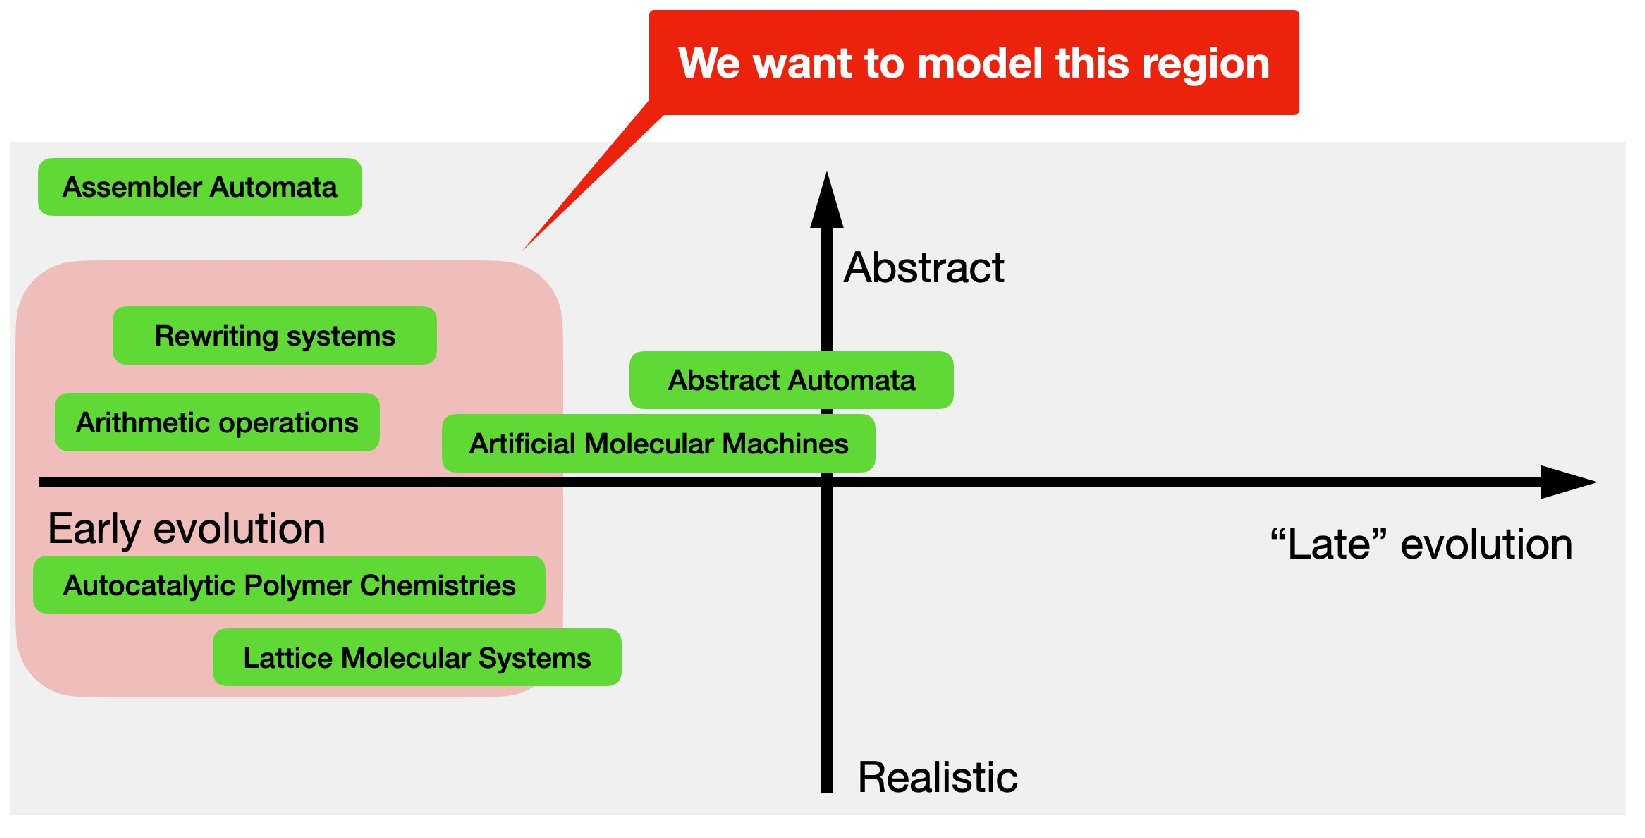
\includegraphics[width=0.90\textwidth]{figures/system/abstraction-stage.pdf}
  \caption{Classification of AC approaches along two axis: abstract vs realistic, and early vs late evolution. In the context of this project we will be focusing on the early evolution, using a balanced approach between more abstract and more realistic models.}
  \label{fig:abstraction-stage}
\end{figure}

The underlying (artificial) chemistry is based on several transformations: formard reactions, backward reactions, diffusion (Table~\ref{tab:reactions}). These reactions are parametrized by rate coefficients ($k_f$, $k_b$, $k_d$). Several other parameters can be defined, such as simulations (temporal) length $\tau_{max}$, the number of reactors $N$, the number of inflows $n$, total mass $M$, etc.

\begin{table}[h]
\centering
\begin{tabular}{|c|c|}
\hline Forward reaction & $A+B \xrightarrow{k_f} C$ \\
\hline Backward reaction & $C \xrightarrow{k_b} A^{\prime}+B$ \\
\hline \multirow{2}{*}{ Diffusion } & $C \xrightarrow{k_d} \varnothing$ \\
\cline { 2 - 2 } & $C_i \xleftrightarrow{k_d} C_j$ \\
\hline
\end{tabular}  
\caption{Reactions occurring in the artificial chemistry implemented in this system. Forward (constructive) reactions happens at rate $k_f$, backward (destructive) reactions happen at rate $k_b$ and diffusion (where a molecule is shifted either to the next chemostat or out of the system) happens at rate $k_d$. Mass $M$ is fixed, so the in-flow is coupled with the diffusion parameter.}
\label{tab:reactions}
\end{table}

\section{System of reactors}

These transformations are applied on a population of integers. These integers form a well-mixed system, inside a reactor/chemostat (Fig.~\ref{fig:reactor-ensemble}a). The number of integers \#1 is fixed, which translates into a fixed in-flow in the first reactor (as these integers are used to form other, more complex integers, or diffuse to the next chemostats). The system as a whole consists of several of these reactors, coupled together via in- and out-flows (defined by the corresponding rates), in a specific topology. For example, one of the simplest topology is that of the regular lattice (Fig.~\ref{fig:reactor-ensemble}b). When diffusion is very high, the whole system becomes well-mixed.

\begin{figure}[hbt]
  \centering
    {\LARGE Diagram of reactor + ensemble of reactors}\vspace{1em}\\
  \begin{overpic}[width=0.35\textwidth]{figures/system/single-reactor.pdf}\put(-15,85){\textbf{(A)}}\end{overpic}\hspace{0.10\textwidth}
  \begin{overpic}[width=0.40\textwidth]{figures/system/ensemble.pdf}\put(-15,95){\textbf{(B)}}\end{overpic}
  \caption{\textbf{(A)} Single reactor, inside of which a bunch of integers react. In-flow is fixed, i.e. the \# of ones is fixed, and these react according to the reactions described in Table~\ref{tab:reactions}. An out-flow connects the reactor to subsequent chemostats. \textbf{(B)} Network of reactors/chemostats. Displayed is a regular lattice (note that diffusion happens both ways). There is a single in-flow, and a single out-flow. Other topologies are possible (see Fig.~\ref{fig:topologies} below.)}
  \label{fig:reactor-ensemble}
\end{figure}

\section{Topologies}

Several topologies can be used to connect the reactors together (Fig.~\ref{fig:topologies}). Examples include: path, lattice, Erdos-Renyi (random), regular (uniform node degree) or Barabasi-Albert (power-law degree distribution). This is especially relevant given that we’re studying living systems, whose networks have been shown to possess certain specific properties deriving from their topology (e.g., resilience from BA networks, etc.) Other topologies (e.g. lattice, random) can be used as control/neutral.

\begin{figure}[hbt]
  \centering
    {\LARGE Examples of topologies}\vspace{1em}\\
  \begin{overpic}[width=0.05\textwidth]{figures/system/graph-path.pdf}\put(-15,95){\textbf{(A)}}\end{overpic}
  \hspace{0.30\textwidth}
  \begin{overpic}[width=0.20\textwidth]{figures/system/graph-lattice.pdf}\put(-15,100){\textbf{(B)}}\end{overpic}\\
  \begin{overpic}[width=0.25\textwidth]{figures/system/graph-ER.pdf}\put(-5,80){\textbf{(C)}}\end{overpic}
  \hspace{0.05\textwidth}
  \begin{overpic}[width=0.25\textwidth]{figures/system/graph-regular.pdf}\put(-15,80){\textbf{(D)}}\end{overpic}
  \hspace{0.05\textwidth}
  \begin{overpic}[width=0.25\textwidth]{figures/system/graph-BA.pdf}\put(-5,80){\textbf{(E)}}\end{overpic}
  \caption{Illustrations of the different topologies we’ll be exploring (at least, in the near future). The chemostats can be connected according to any of these topologies, which we presume will affect the construction of molecular complexity in the mixture. \textbf{(A)} Simple path lattice. \textbf{(B)} Lattice. \textbf{(C)} Random (Erdos-Rényi) graph. \textbf{(D)} Regular graph (all nodes have the same degree). \textbf{(E)} Scale-free (Barabasi-Albert) graph, with the distribution of nodes follow a power law.}
  \label{fig:topologies}
\end{figure}

\section{Integer chemistry and Assembly Theory}

We’ll be using Assembly Theory to quantify the complexity emerging from the mixture, therefore we’ll use the Assembly Index ($A$). Cole has calculated $A$ for integers $<10000$. The Assembly Index increases as the logarithm of integer values (Fig.~\ref{fig:integers-assembly}). We’ll however probably be using both, as some relationships are better illustrated using y-axis as integers, and others with the y-axis as the Assembly Index.

\begin{figure}[hbt]
  \centering
  {\LARGE Relationship integers vs. assembly index}\vspace{1em}\\
  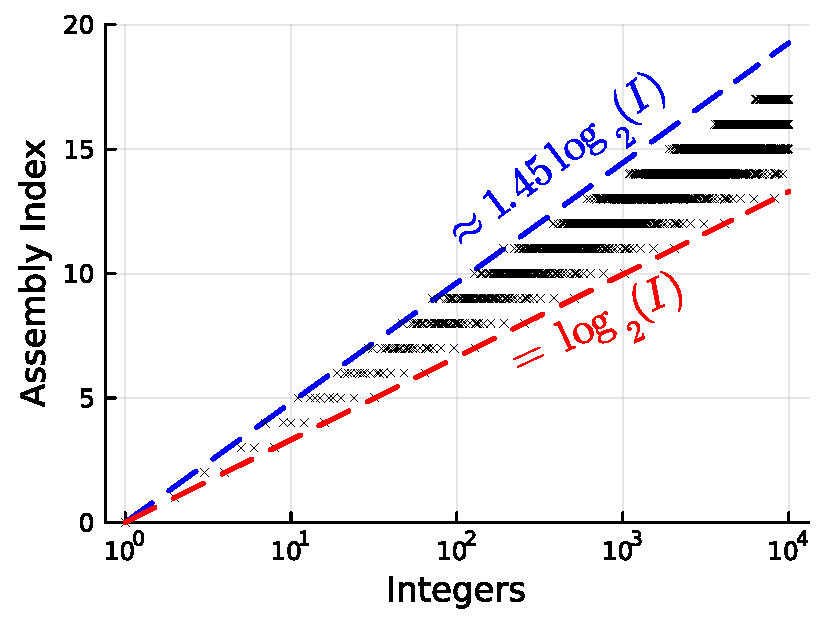
\includegraphics[width=0.40\textwidth]{figures/system/integers-assembly.pdf}
  \caption{Assembly Index $A$ for integers $<10000$. $A$ increases as the logarithm of integer values.}
  \label{fig:integers-assembly}
\end{figure}

\chapter{Experiments}

\section{MS01: time series}

A first result we can plot using this system is the time series of the populations (shown on Fig.~\ref{fig:time-series}). The layout of this figure follows the same structure as the one on Fig.~\ref{fig:reactor-ensemble}b: each panel shows the evolution of integers $I\in{1...10}$ through time. The blue curve shows ones, we can see the number of ones is fixed on the first panel (top left). Diffusion pushes molecules to the next chemostats that are connected to the first one (where the in-flow is) so we’re seeing initial transients/peaks at different times. The higher we increase diffusion, the faster these peaks happen, and the shorter is the initial transient.

\begin{figure}[hbt]
  \centering
  {\LARGE Example of time series for an ensemble of reactors}\vspace{1em}\\
  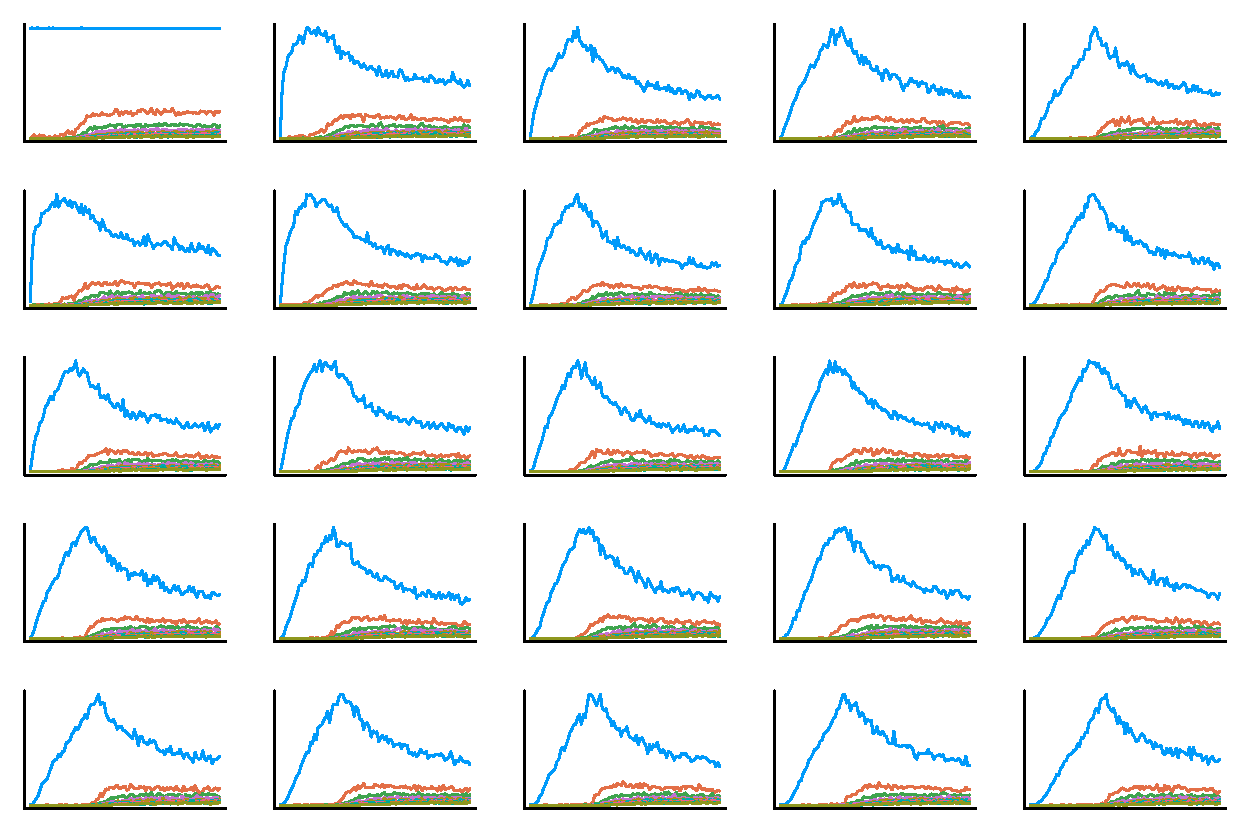
\includegraphics[width=0.75\textwidth]{figures/results/1-prelim/ts-gridplot.pdf}
  \caption{Time series for a simulation of 25 chemostats connected in a regular lattice. The first panel (top left) corresponds to the chemostat with an in-flow connected to it. The ten first species (integers $I\in{1...10}$) are shown.}
  \label{fig:time-series}
\end{figure}

\clearpage

\section{MS02: varying the diffusion rate}

A first parameter we’re exploring is the diffusion rate. We’ve sampled simulations with diffusion rates $k_d\in[10^{-6},10^{2}$ and plot the first ten species (excluding ones) on Fig.~\ref{fig:prelim-abundance}. Panel A shows the average populations across reactors, i.e. taking all the chemostats together as one single population and calculating the average for species $S$ at the last iteration of the simulation $\tau_{max}$. We’ve done this calculation for 100 values of $k_d$ (without using statistical ensembles for now). The shaded area on Panel A represents the standard deviation across chemostats, and is also illustrated on Panel B. We’ve also added a vertical (dashed) line to indicade the forward rate $k_f$. 

One thing we can readily notice from Fig.~\ref{fig:prelim-diffusion} is the presence of transitions. On Panel A we have four regimes: low values in the populations of complex (i.e. $I>1$) species for lower values of the diffusion coefficient ($k_d < k_f$), then increasing complexity ($k_f < k_d < 1$), then a dip in complexity ($k_d ~ 10$), and finally complexity increasing again for very high diffusion rates ($k_d \gtrsim 10^2$). Panel B shows an increase in $\sigma$ until $k_d ~ 10^{-1}$ then a sharp decrease ($10^{-1} < k_d < 10$).

\begin{figure}[hbt]
  \vspace{2em}
  \centering
  {\LARGE Populations (and their std) across diffusion rates}\vspace{3em}\\
  \begin{overpic}[width=0.45\textwidth]{figures/results/1-prelim/mu-vs-kd.pdf}\put(-5,80){\textbf{(A)}}\end{overpic}
  \begin{overpic}[width=0.45\textwidth]{figures/results/1-prelim/sd-vs-kd.pdf}\put(-5,80){\textbf{(B)}}\end{overpic}
  \caption{\textbf{(A)} Average populations, calculated across all chemostats, at $\tau_{max}$ for the first ten integers excluding ones. Shaded area represents the standard deviation (also pictured on Panel B). \textbf{(B)} Standard deviation for the same species shown on Panel A.}
  \label{fig:prelim-diffusion}
\end{figure}

Another thing we can calculate from these systems is the total mass, i.e. $I_i \times f_i$ (where $I_i$ is the integer of species $i$ and $f_i$ the number of identical copies or "copy number"). Shown on Fig.~\ref{fig:prelim-diffusion} is the total mass $M$ against the same variation in coefficient discussed above. $M$ stays constant for most values of the diffusion coefficient but increases exponentially for the highest values of $k_d$.\\

\begin{figure}[hbt]
  \centering
  {\LARGE Total mass of the system vs diffusion coefficient}\vspace{1em}\\
  \begin{overpic}[width=0.45\textwidth]{figures/results/1-prelim/mass.pdf}\end{overpic} \\
  \caption{Increase in total mass as we increase diffusion. Total mass $M$ is calculated by multiplying integers $I_i$ with their copy number $f_i$.}
  \label{fig:prelim-mass}
\end{figure}

\note{Putting this all together:}{There seems to be three regimes based on what we’re seeng in Figs~\ref{fig:prelim-diffusion}-\ref{fig:prelim-mass}: initially, we have a well-mixed system in the first chemostat. The complexity in chemostat \#1 increases, but all other chemostats remain empty, which is why we’re seeing low average values in Fig.~\ref{fig:prelim-diffusion} (they’re calculated over all chemostats). Then, as we increase diffusion the other chemostats are progressively filled up: this is why the standard deviation increases. Finally, as all chemostats are fully filled and we continue increasing the diffusion, the system returns to a well-mixed state and the mass increases rapidly (because complexity now builds up in all the chemostats).}

\clearpage

\section{MS03: measuring distance from source}

One additional experiment we’ve done was to investigate how the mean assembly index (per reactor) varied with the distance from source $D$. For example, the distance $D$ between the source (in green) and the target chemostat (in red) shown on Fig.~\ref{fig:prelim-distance}a would be six. We’ve evaluated how the complexity varied with $D$ for three diffusion regimes: low diffusion ($k_d=10^{-4}$), intermediate diffusion ($k_d = 10^{-2}$) and high diffusion ($k_d=10$). Complex molecules remain in the chemostats that are located close to the source $D=1,2$ when diffusion is low (Fig.~\ref{fig:prelim-distance}, blue curve) or intermediary (red curve). When diffusion is increased (green curve), complexity spreads to the other reactors.

However, there remains a degeneracy when we examine the complexity contained in chemostats located at identical distances from the source (Fig.~\ref{fig:prelim-distance}, dashed box surrounding data points at $D=5$). Multiple chemostats at $D=5$ have different (average values of the) assembly index. This is clearly evident when looking at the inset in Fig.~\ref{fig:prelim-distance} that displays the density plots (i.e., reconstructed PDF): the heavy tails extending to high values of $A$ clearly differ from one chemostat to another. Consequently, $D$ alone does not fully determine the quantitative complexity of the mixture.

\begin{figure}[hbt]
  \centering
  \hspace{2em}
  {\LARGE Mean assembly index vs distance from the source}\vspace{1em}\\
  \begin{overpic}[width=0.33\textwidth]{figures/results/1-prelim/ensemble-distance.pdf}\put(-15,80){\textbf{(A)}}\end{overpic}
  \hspace{0.10\textwidth}
  \begin{overpic}[width=0.40\textwidth]{figures/results/1-prelim/AI-vs-D.pdf}\put(-5,70){\textbf{(B)}}\end{overpic}
  \caption{\textbf{(A)} Here we investigate how complexity varies as a function of the distance $D$ from the source. For example, the distance between the in-flow (green) and the target chemostat (red) is six. \textbf{(B)} Complexity as a function of the distance from the source, for three diffusion regimes. Inset: density plots for the four chemostats having $D=5$. Clearly, $D$ alone does not fully determine the complexity of the mixture.}
  \label{fig:prelim-distance}
\end{figure}

\clearpage

\section{MS04: measuring detection thresholds}

Next, we want to relate these experiments to observational missions by evaluating thresholds in complexity that we could detect. We can therefore evaluate the abundance of the different species (i.e., populations as a fraction of total \# of molecules or total mass---here we chose the former) and determine the most complex molecule we could detect using an instrument capable of measuring concentrations of $10^{-5}$ (i.e. 1 molecule in a system having a total of $10^5$ molecules), then $10^{-4}$, and so on. Fig.~\ref{fig:prelim-abundance} how the complexity of detectable molecules varies as we change the diffusion coefficient.

\begin{figure}[hbt]
  \centering
  {\LARGE Detection thresholds vs diffusion coefficient}\vspace{1em}\\
  \begin{overpic}[width=0.40\textwidth]{figures/results/1-prelim/abundance-I.pdf}\put(-5,70){\textbf{(A)}}\end{overpic}
  \hspace{0.05\textwidth}
  \begin{overpic}[width=0.40\textwidth]{figures/results/1-prelim/abundance-A.pdf}\put(-5,70){\textbf{(B)}}\end{overpic}
  \caption{\textbf{(A)} Most complex detectable molecule for different thresholds (indicated in the legend) as we vary the diffusion rate. Raw integer values are shown. \textbf{(B)} Same as Panel A, but the Assembly Index is used instead to indicate the complexity of the molecules.}
  \label{fig:prelim-abundance}
\end{figure}

In Fig.~\ref{fig:prelim-abundance}, on Panel A we plot the raw integer values against $k_d$ whereas on Panel B we’re showing the assembly index instead. We’re using five different detection thresholds ($10^{-5},\cdots,10^{-1}$). Each data point indicates the integer value (or assembly index) of the most complex molecule that’s detectable using this specific threshold. Going back to what we mentioned previously about transitions and regimes, we can now clearly see the three regimes we talked about in Fig.~\ref{fig:prelim-abundance}: for lower values of $k_d$, all the complexity is contained in the first chemostat and we’re just sampling the heavy tails, as we increase diffusion the molecules spread in the other chemostats and complexity suddenly decreases, finally as we further increase $k_d$ complexity rises again.

Basically, we have two competing phenomena: (1) increasing complexity as we increase $k_d$, but also (2) decreased ability to detect the molecules when they spread initially (which decreases their concentration)---until they have filled all the chemostats and their concentration increases again. This is why we’re seeing a minima on Fig.~\ref{fig:prelim-abundance}: this point represents the area of the parameter space where the molecules are in the process of filling up the chemostats.

\paragraph{Upcoming experiments}

Some things we are considering:

\begin{itemize}
	\item making a figure of the "cones" which define assembly spaces for graphs/integers/molecules (similar to the one in Fig.~\ref{fig:assembly-cones} below)
	\item decoupling in-flow and diffusion: right now in-flow is implicit, i.e. we have a fixed number of ones in chemostat \#1, and when we increase diffusion we push molecules to the next chemostats (which amounts to refilling chemostat \#1, since the number of ones is fixed). This prevents us from increasing the in-flow independently from the diffusion coefficient, which could increase complexity without increasing diffusion so much (making the whole system a giant well-mixed system, and also making the simulations much longer to compute)
\end{itemize}

\begin{figure}[hbt]
  \centering
  {\LARGE Assembly spaces (Sharma 2023)}\vspace{1em}\\
  \begin{overpic}[width=0.60\textwidth]{figures/results/1-prelim/assembly-cones.pdf}\end{overpic}
  \caption{Cones defining the different assembly spaces. Taken from \cite{sharma_assembly_2023}.}
  \label{fig:assembly-cones}
\end{figure}

\clearpage

\section{MS06: implementing tau-leaping}

{\color{blue}\lipsum}

\clearpage

\section{MS08: distance from source (bis)}

{\color{blue}\lipsum}

\begin{figure}[ht]
  \centering
  {\LARGE Mean AI vs distance from the source (recoded in R)}\vspace{1em}\\
  \begin{overpic}[width=0.45\textwidth]{figures/results/MS08/08C_distance-from-source}
%  	\put(-5,80){\textbf{(A)}}
  \end{overpic}
  \caption{\textbf{(A)} ...}
  \label{fig:}
\end{figure}

\clearpage

\section{MS09: varying diffusion (bis)}

{\color{blue}\lipsum}

\begin{figure}[hbt]
  \centering
  {\LARGE Populations and their std vs diffusion rate (recoded in R)}\vspace{1em}\\
  \begin{overpic}[width=0.45\textwidth]{figures/results/MS09/09C_mean-populations-across-kd}
  	\put(-5,80){\textbf{(A)}}
  \end{overpic}
  \begin{overpic}[width=0.45\textwidth]{figures/results/MS09/09C_sd-populations-across-kd}
  	\put(-5,80){\textbf{(B)}}
  \end{overpic}
  \caption{\textbf{(A)} ...}
  \label{fig:}
\end{figure}

\begin{figure}[hbt]
  \centering
  {\LARGE Detection thresholds vs diffusion (recoded in R)}\vspace{1em}\\
  \begin{overpic}[width=0.45\textwidth]{figures/results/MS09/09C_detection_thresholds_int}
  	\put(-5,80){\textbf{(A)}}
  \end{overpic}
  \begin{overpic}[width=0.45\textwidth]{figures/results/MS09/09C_detection_thresholds_AI}
  	\put(-5,80){\textbf{(B)}}
  \end{overpic}
  \caption{\textbf{(A)} ...}
  \label{fig:}
\end{figure}

\clearpage

\section{MS12: assembly of integers (bis)}

{\color{blue}\lipsum}

\begin{figure}[hbt]
  \centering
  {\LARGE Integer value and assembly index (recoded in R)}\vspace{1em}\\
  \begin{overpic}[width=0.45\textwidth]{figures/results/MS12/12_assembly-of-integers}
%  	\put(-5,80){\textbf{(A)}}
  \end{overpic}
  \caption{\textbf{(A)} ...}
  \label{fig:}
\end{figure}

\clearpage

\section{MS13: integers histogram}

{\color{blue}\lipsum}

\begin{figure}[hbt]
  \centering
  {\LARGE Distribution of integers/AIs for a whole system}\vspace{1em}\\
  \begin{overpic}[width=0.45\textwidth]{figures/results/MS13/13_integers-histogram}
%  	\put(-5,80){\textbf{(A)}}
  \end{overpic}
  \caption{\textbf{(A)} ...}
  \label{fig:}
\end{figure}

\clearpage

\section{MS15-18: sweep on inflow $\times$ diffusion with $t_\text{max}=10^2, 10^3, 10^4$}

{\color{blue}\lipsum}

\begin{figure}[hbt]
  \centering
  {\LARGE Time series for a single simulation and for whole systems}\vspace{1em}\\
  \vspace{3em}
  \begin{overpic}[width=0.33\textwidth]{figures/results/MS15/single-timeseries}
  \put(30,110){\huge $t_\text{max}=10^2$}
  	\put(-5,95){\textbf{(A)}}
  \end{overpic}
  \begin{overpic}[width=0.33\textwidth]{figures/results/MS17/single-timeseries}
    \put(30,110){\huge $t_\text{max}=10^4$}
  	\put(-5,95){\textbf{(B)}}
  \end{overpic}
  \begin{overpic}[width=0.33\textwidth]{figures/results/MS18/single-timeseries_62}
    \put(30,110){\huge $t_\text{max}=10^4$}
  	\put(-5,95){\textbf{(C)}}
  \end{overpic}
  \begin{overpic}[width=0.33\textwidth]{figures/results/MS15/multipanel-timeseries}
  	\put(-5,95){\textbf{(D)}}
  \end{overpic}
  \begin{overpic}[width=0.33\textwidth]{figures/results/MS17/multipanel-timeseries}
  	\put(-5,95){\textbf{(E)}}
  \end{overpic}
  \begin{overpic}[width=0.33\textwidth]{figures/results/MS18/multipanel-timeseries}
  	\put(-5,95){\textbf{(F)}}
  \end{overpic}
  \caption{\textbf{(A)} ...}
  \label{fig:}
\end{figure}

\begin{figure}[hbt]
  \centering
  {\LARGE Power law fit over the whole system (integer/AI) and inflow/outflow}\vspace{1em}\\
  \vspace{3em}
  \begin{overpic}[width=0.33\textwidth]{figures/results/MS15/multipanel-histograms}
    \put(30,110){\huge $t_\text{max}=10^2$}
  	\put(-5,95){\textbf{(A)}}
  \end{overpic}
  \begin{overpic}[width=0.33\textwidth]{figures/results/MS17/multipanel-histograms}
    \put(30,110){\huge $t_\text{max}=10^3$}
  	\put(-5,95){\textbf{(B)}}
  \end{overpic}
  \begin{overpic}[width=0.33\textwidth]{figures/results/MS18/multipanel-histograms}
    \put(30,110){\huge $t_\text{max}=10^4$}
  	\put(-5,95){\textbf{(C)}}
  \end{overpic}
  \begin{overpic}[width=0.33\textwidth]{figures/results/MS15/multipanel-histograms-AI}
  	\put(-5,95){\textbf{(D)}}
  \end{overpic}
  \begin{overpic}[width=0.33\textwidth]{figures/results/MS17/multipanel-histograms-AI}
  	\put(-5,95){\textbf{(E)}}
  \end{overpic}
  \begin{overpic}[width=0.33\textwidth]{figures/results/MS18/multipanel-histograms-AI}
  	\put(-5,95){\textbf{(F)}}
  \end{overpic}
  \begin{overpic}[width=0.33\textwidth]{figures/results/MS15/multipanel-histograms-inflow-outflow}
  	\put(-5,95){\textbf{(G)}}
  \end{overpic}
  \begin{overpic}[width=0.33\textwidth]{figures/results/MS17/multipanel-histograms-inflow-outflow}
  	\put(-5,95){\textbf{(H)}}
  \end{overpic}
  \begin{overpic}[width=0.33\textwidth]{figures/results/MS18/multipanel-histograms-inflow-outflow}
  	\put(-5,95){\textbf{(I)}}
  \end{overpic}
  \caption{\textbf{(A)} ...}
  \label{fig:}
\end{figure}

\begin{figure}[hbt]
  \centering
  {\LARGE Exponent of power law fit, average integer and total mass}\vspace{1em}\\
  \vspace{3em}
  \begin{overpic}[width=0.32\textwidth]{figures/results/MS15/heatmap-exponents-linear}
    \put(30,100){\huge $t_\text{max}=10^2$}
  	\put(-5,85){\textbf{(A)}}
  \end{overpic}
  \begin{overpic}[width=0.32\textwidth]{figures/results/MS17/heatmap-exponents-linear}
    \put(30,100){\huge $t_\text{max}=10^3$}
  	\put(-5,85){\textbf{(B)}}
  \end{overpic}
  \begin{overpic}[width=0.32\textwidth]{figures/results/MS18/heatmap-exponents-linear}
    \put(30,100){\huge $t_\text{max}=10^4$}
  	\put(-5,85){\textbf{(C)}}
  \end{overpic}
  \begin{overpic}[width=0.32\textwidth]{figures/results/MS15/heatmap-avg-integer-log}
  	\put(-5,85){\textbf{(D)}}
  \end{overpic}
  \begin{overpic}[width=0.32\textwidth]{figures/results/MS17/heatmap-avg-integer-log}
  	\put(-5,85){\textbf{(E)}}
  \end{overpic}
  \begin{overpic}[width=0.32\textwidth]{figures/results/MS18/heatmap-avg-integer-log}
  	\put(-5,85){\textbf{(F)}}
  \end{overpic}
  \begin{overpic}[width=0.32\textwidth]{figures/results/MS15/heatmap-total-mass-log}
  	\put(-5,85){\textbf{(G)}}
  \end{overpic}
  \begin{overpic}[width=0.32\textwidth]{figures/results/MS17/heatmap-total-mass-log}
  	\put(-5,85){\textbf{(H)}}
  \end{overpic}
  \begin{overpic}[width=0.32\textwidth]{figures/results/MS18/heatmap-total-mass-log}
  	\put(-5,85){\textbf{(I)}}
  \end{overpic}
  \caption{\textbf{(A)} ...}
  \label{fig:}
\end{figure}

\begin{figure}[hbt]
  \centering
  {\LARGE Exponents of power law fit at inflow/outflow/diff ($t_\text{max}=10^4$)}\vspace{1em}\\
  \begin{overpic}[width=0.32\textwidth]{figures/results/MS18/heatmap-exponents-inflow}
  	\put(-5,85){\textbf{(A)}}
  \end{overpic}
  \begin{overpic}[width=0.32\textwidth]{figures/results/MS18/heatmap-exponents-outflow}
  	\put(-5,85){\textbf{(B)}}
  \end{overpic}
  \begin{overpic}[width=0.32\textwidth]{figures/results/MS18/heatmap-exponents-diff}
  	\put(-5,85){\textbf{(C)}}
  \end{overpic}
  \caption{\textbf{(A)} ...}
  \label{fig:}
\end{figure}

\begin{figure}[hbt]
  \centering
  {\LARGE Time series for limit cases ($t_\text{max}=10^4$)}\vspace{1em}\\
  \begin{overpic}[width=0.45\textwidth]{figures/results/MS18/single-timeseries_1}
    \put(80,110){\huge }
  	\put(-5,95){\textbf{(A)}}
  \end{overpic}
   \begin{overpic}[width=0.45\textwidth]{figures/results/MS18/single-timeseries_10}
  	\put(-5,95){\textbf{(B)}}
  \end{overpic}
   \begin{overpic}[width=0.45\textwidth]{figures/results/MS18/single-timeseries_91}
  	\put(-5,95){\textbf{(C)}}
  \end{overpic}
   \begin{overpic}[width=0.45\textwidth]{figures/results/MS18/single-timeseries_100}
  	\put(-5,95){\textbf{(D)}}
  \end{overpic}
  \caption{\textbf{(A)} ...}
  \label{fig:}
\end{figure}

\clearpage

\section{MS16: numerical stability test aka testing $dt$}

{\color{blue}\lipsum}

\clearpage

\section{Wrapping up MS15-18}

%- time series chemostats (limit cases)
%- histograms exp fits inflow/outflow
%- heatmaps exponents inflow/outflow/diff
%- heatmaps avg integer (log scale)
%- heatmaps mass (log scale)

%\begin{figure}[hbt]
%  \centering
%  {\LARGE Time series for limit cases}\vspace{1em}\\
%  \begin{overpic}[width=0.24\textwidth]{figures/results/MS18/single-timeseries_1}
%    \put(80,110){\huge }
%  	\put(-5,95){\textbf{(A)}}
%  \end{overpic}
%   \begin{overpic}[width=0.24\textwidth]{figures/results/MS18/single-timeseries_10}
%  	\put(-5,95){\textbf{(B)}}
%  \end{overpic}
%   \begin{overpic}[width=0.24\textwidth]{figures/results/MS18/single-timeseries_91}
%  	\put(-5,95){\textbf{(C)}}
%  \end{overpic}
%   \begin{overpic}[width=0.24\textwidth]{figures/results/MS18/single-timeseries_100}
%  	\put(-5,95){\textbf{(D)}}
%  \end{overpic}
%  \vskip1em
%  {\LARGE Power law fit and exponents at inflow/outflow/diff}\vspace{0em}\\
%  \begin{overpic}[width=0.24\textwidth]{figures/results/MS18/multipanel-histograms-inflow-outflow}
%  	\put(-5,95){\textbf{(E)}}
%  \end{overpic}
%  \begin{overpic}[width=0.24\textwidth]{figures/results/MS18/heatmap-exponents-inflow}
%  	\put(-5,85){\textbf{(F)}}
%  \end{overpic}
%  \begin{overpic}[width=0.24\textwidth]{figures/results/MS18/heatmap-exponents-outflow}
%  	\put(-5,85){\textbf{(G)}}
%  \end{overpic}
%  \begin{overpic}[width=0.24\textwidth]{figures/results/MS18/heatmap-exponents-diff}
%  	\put(-5,85){\textbf{(H)}}
%  \end{overpic}
%  \vskip1em
%  {\LARGE Average integer and total mass}\vspace{1em}\\
%  \begin{overpic}[width=0.32\textwidth]{figures/results/MS18/heatmap-avg-integer-log}
%  	\put(-5,85){\textbf{(I)}}
%  \end{overpic}
%  \begin{overpic}[width=0.32\textwidth]{figures/results/MS18/heatmap-total-mass-log}
%  	\put(-5,85){\textbf{(J)}}
%  \end{overpic}
%  \caption{\textbf{(A)} ...}
%  \label{fig:}
%\end{figure}

\begin{figure}[hbt]
  \centering
\begin{minipage}{0.5\linewidth}
\centering
{\LARGE Time series for limit cases}\vspace{1em}\\
  \begin{overpic}[width=0.49\textwidth]{figures/results/MS18/single-timeseries_1}
    \put(80,110){\huge }
    \put(-5,95){\textbf{(A)}}
  \end{overpic}
  \begin{overpic}[width=0.49\textwidth]{figures/results/MS18/single-timeseries_10}
    \put(-5,95){\textbf{(B)}}
  \end{overpic}
  \begin{overpic}[width=0.49\textwidth]{figures/results/MS18/single-timeseries_91}
    \put(-5,95){\textbf{(C)}}
  \end{overpic}
  \begin{overpic}[width=0.49\textwidth]{figures/results/MS18/single-timeseries_100}
    \put(-5,95){\textbf{(D)}}
  \end{overpic}
\end{minipage}
\begin{minipage}{0.49\linewidth}	
\centering
{\Large Power law fits over inflow/outflow}\vspace{1em}\\
  \begin{overpic}[width=0.99\textwidth]{figures/results/MS18/multipanel-histograms-inflow-outflow}
  	\put(-0,95){\textbf{(E)}}
  \end{overpic}
\end{minipage}

  \vskip1em
  {\LARGE Exponents of power law fits at inflow/outflow/diff}\vspace{1em}\\
  \begin{overpic}[width=0.32\textwidth]{figures/results/MS18/heatmap-exponents-inflow}
  	\put(-5,85){\textbf{(F)}}
  \end{overpic}
  \begin{overpic}[width=0.32\textwidth]{figures/results/MS18/heatmap-exponents-outflow}
  	\put(-5,85){\textbf{(G)}}
  \end{overpic}
  \begin{overpic}[width=0.32\textwidth]{figures/results/MS18/heatmap-exponents-diff}
  	\put(-5,85){\textbf{(H)}}
  \end{overpic}
  \vskip1em
  {\LARGE Average integer and total mass}\vspace{1em}\\
  \begin{overpic}[width=0.32\textwidth]{figures/results/MS18/heatmap-avg-integer-log}
  	\put(-5,85){\textbf{(I)}}
  \end{overpic}
  \begin{overpic}[width=0.32\textwidth]{figures/results/MS18/heatmap-total-mass-log}
  	\put(-5,85){\textbf{(J)}}
  \end{overpic}
  \caption{\textbf{(A)} ...}
  \label{fig:}
\end{figure}

\clearpage

\section{MS19: varying the topology}

%\chapter{References}
%\bibliographystyle{apalike}
\footnotesize
\setlength{\bibsep}{0.0pt}
\bibliography{references-new.bib}

\end{document}
